
\section{Синтаксический анализатор}
Парсер выполняет преобразование текста, записанного на языке Пролог, во внутреннее представление, удобное для дальнейшей работы. Синтаксический анализатор разработан с использование библиотеки \texttt{parsec}.

Для разработки синтаксического анализатора требовалось описать грамматику языка при помощи типов.

\lstinputlisting[caption = {Описание программы}, label={lst1:syntax},language=Haskell, firstline=6, lastline=37]{../src/Language/Prolog/Syntax.hs}

Чтобы разобрать текст программы, необходимо описать, как разобрать любую его структуру. Например, при помощи пакета \texttt{parsec}, чтобы проверить, является ли строка числом, необходимо написать следующий код, представленный в листинге \ref{lst2:syntax}.

\lstinputlisting[caption = {Парсер целого числа}, label={lst2:syntax},language=Haskell, firstline=214, lastline=225]{../src/Language/Prolog/Parser.hs}

В листинге \ref{lst3:syntax} представлен код, необходимый, чтобы получить число, как описанный в листинге \ref{lst2:syntax} тип.

\lstinputlisting[caption = {Парсер структуры языка}, label={lst3:syntax},language=Haskell, firstline=16, lastline=32]{../src/Language/Prolog/Parser.hs}

Подобные действия необходимо выполнить для каждого типа.

\section{Алгоритм унификации}
Алгоритм унификации на языке Haskell представлен в листинге \ref{lst4:unifi}.
\lstinputlisting[caption = {Алгоритм унификации}, label={lst4:unifi},language=Haskell, firstline=317, lastline=332]{../src/Language/Prolog/Algorithm.hs}

Функция принимает в качестве аргументов два терма. Возвращаемым значением, в случае успешной унификации, будет новая цель или подстановка.

\section{Доказательство}
В листинге \ref{lst4:proof} показан шаг обработки текущей цели.
\lstinputlisting[caption = {Доказательство}, label={lst4:proof},language=Haskell, firstline=112, lastline=145]{../src/Language/Prolog/Algorithm.hs}

В первую очередь проверяется резольвента. Если она пуста, то возвращается выработанная подстановка. Если все цели из текущего правила закончились, то переход к целям из тела следующего правила.
Если встречено отсечение, то продолжается поиск решений в данной ветке, но вместе с найденными результатами возвращается метка отсечения.
Далее вызывается обработчик для текущего терма. Стандартный обработчик, представлен в листинге \ref{lst4:default}.
\lstinputlisting[caption = {Стандартный обработчик}, label={lst4:default},language=Haskell, firstline=206, lastline=233]{../src/Language/Prolog/Algorithm.hs}

В данном обработчике выполняется попытка унификации текущей цели со всеми возможными правилами. В случае успешной унификации происходит преобразование резольвенты для каждой отдельной ветки. Если в какой-то момент встречается метка отсечения, и она соответствует текущему терму, то следующие ветки в списке отбрасываются.

\section{Отсечение}
Для работы алгоритма, в качестве хранилища контрольных точек, было выбрано дерево. Такой выбор был сделан для простоты визуализации дерева поиска решений. Позже оказалось, что данная структура не подходит для работы алгоритма. Если отсечения стоит в середине тела правила, то откат может быть совершен в обратную сторону по отсечению. В результате этого корректная работа программы возможно только в случае, если отсечение стоит в конце предложения или если его нет. В противном случае, программа может работать некорректно. 

Был сделан вывод, что для дальнейшей разработки лучше использовать стек, который хранит текущую подстановку, резольвенту и возможные варианты ветвления. Но при данной конфигурации значительно усложняется алгоритм построения дерева поиска решений.

\section{Генерация изображений}
Graphviz -- пакет утилит по автоматической визуализации графов, заданных в виде описания на языке DOT, а также дополнительных текстовых и графических программ, виджетов и библиотек, используемых при разработке программного обеспечения для визуализации структурированных данных. В данной работе использовался Graphviz для генерации изображний.

\section{Примеры работы программы}
Для программы нахождения факториала, приведенной в листинге \ref{lst:pr1}, построено дерево, изображенное на рисунке  \ref{uc:1}.
\lstinputlisting[caption = {Факториал}, label={lst:pr1},language=Prolog]{../p1.pro}
\begin{figure}[H]
	\centering{ 
		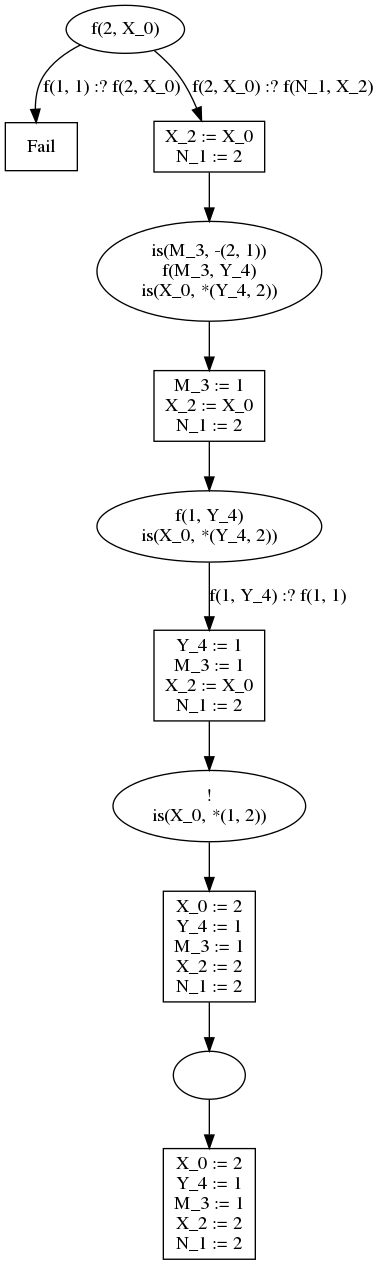
\includegraphics[width=0.4\textwidth]{../fact.png}
		\caption{Дерево поиска решения для факториала}
		\label{uc:1}}
	\end{figure}

\newpage
Для программы соединения двух списков, приведенной в листинге \ref{lst:pr2}, построено дерево, изображенное на рисунке \ref{uc:2}.
\lstinputlisting[caption = {Append}, label={lst:pr2},language=Prolog]{../p2.pro}
\begin{figure}[H]
\centering{ 
	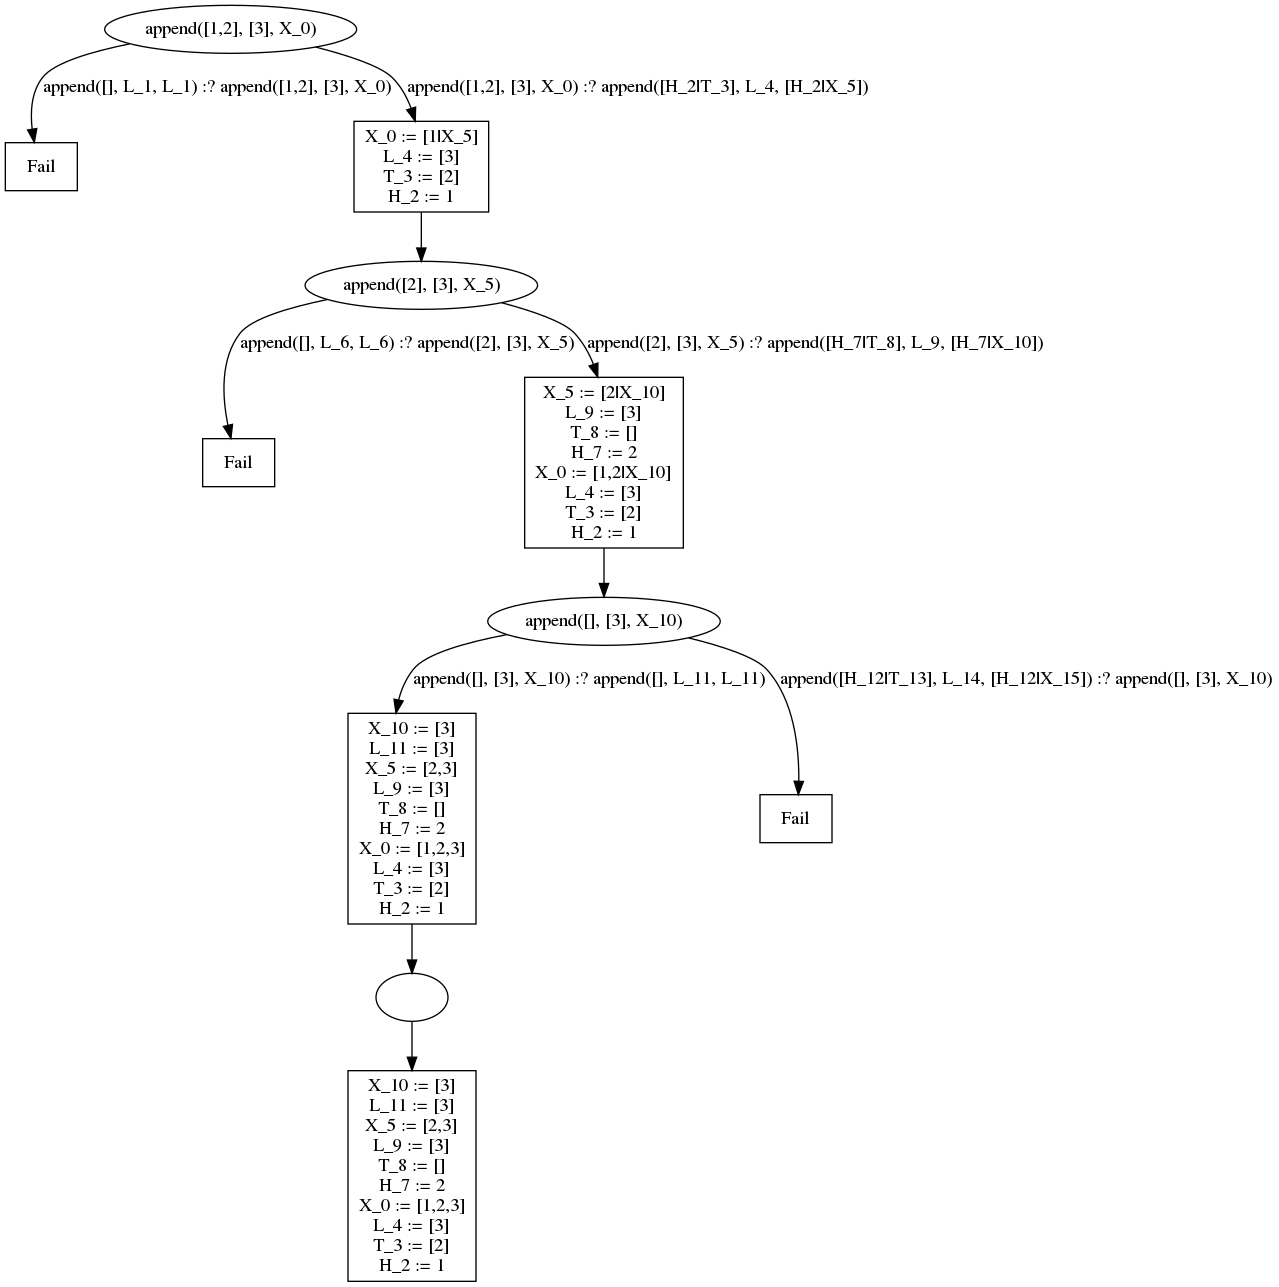
\includegraphics[width=\textwidth]{../t3.png}
	\caption{Дерево поиска решения для соединения списков}
	\label{uc:2}}
\end{figure}
 
